\documentclass{article}
\usepackage{epsfig}
\usepackage{graphicx}
\usepackage[table]{xcolor}
\title{CS345 Theoretical Assignment 1 \\ }
\author{\vspace{2mm} \large Ayush Agarwal, 13180 \\ M.Arunothia, 13378}
\date{}
\begin{document}
\maketitle
\tableofcontents
\newpage
\section{Non-Dominated Points}
\subsection{Overview}
Given a set of coordinates P, we create list of each layer in the following manner.\\
First sort the coordinates based on Y-coordinate in descending order. Then maintain an array A of size $n$. Start with the first coordinate from 
the sorted array P(of all coordinates). This point will be a non-dominated point and will be a part of layer 1. Update the first index of A with the x-coordinate
of this point. Now take the second point from P. If its x coordinate is greater than the x-coordinate of earlier point, it means that it will be part of layer
1. If so then add it to layer 1 and update the layer 1's index in A. Otherwise it will be in second layer, so add it in layer 2 and update the layer 2's index 
in A with it's x coordinate. Repeat the above procedure for all points.

\subsection{Pseudo-Code}
Non-Dominated-points(P)	\\*
\{			\\*
    \hspace*{1cm}P $\longrightarrow$ reverse_sort(P) //sort in descending order of Y  \\*
    \hspace*{1cm} A[0]=P[0].x \\*
    \hspace*{1cm} Layer[1].push() \\*
	\hspace*{1cm} i=1; right=1 \\*
    \hspace*{1cm}while(i<P.length())\\*
    \hspace*{2cm} point = P[i]\\*
    \hspace*{2cm} index = binary_search_predecessor(A, 0, right, point)\\*
    \hspace*{2cm} Layer[index].push(point)\\*
    \hspace*{2cm} A[index] = point.x\\*
	\\*
\}
\section{ Open Rectangle Query }
\subsection{Data Structure Design : } 
Given an array 'a' of 'n' coordinate points, we construct a Binary Search Tree (BST) call it 'data' in the following manner.\\*
\begin{itemize}
\item Sort the array 'a' w.r.t the x-coordinates of the points. Call this sorted array 'b'.
\item Divide 'b' into $ \frac{n}{Log[n]} $ parts, starting from the beginning. Index each of the part incrementally from 1 to $ \frac{n}{Log[n]} $. 
\item Construct BST 'data' with $ \frac{n}{Log[n]} = N $ nodes from 'b' using the above indexing for the comparisons.
\item Now, we have a BST 'data' with 'N' nodes augmented with an array of $Log[n]$ size at every node. Sort this array at every node on basis of y-coordinates of the points.
\item This completes the description of augmented BST 'data'.
\end{itemize}
\section*{Given Array 'a'}
\hspace{-4.8cm}
\begin{tabular}{ |c|c|c|c|c|c|c|c|c|c|c|c|c|c|c|c|}
\hline
\cellcolor{red} (13,1) & (4,2) & (11,3) & (2,4) & \cellcolor{red} (8,5) & (9,6) & (5,7) & (14,8) & \cellcolor{red} (3,9) & (12,10) & (10,11) & (6,12) & \cellcolor{red} (1,13) & (16,14) & (15,15) & (7,16) \\ \hline
\end{tabular}
\section*{Sorted Array 'b' based on x coordinates}
\hspace{-4.8cm}
\begin{tabular}{ |c|c|c|c|c|c|c|c|c|c|c|c|c|c|c|c|}
\hline
\cellcolor{red} (1,13) & (2,4) & (3,9) & (4,2) & \cellcolor{red} (5,7) & (6,12) & (7,16) & (8,5) & \cellcolor{red} (9,6) & (10,11) & (11,3) & (12,10) & \cellcolor{red} (13,1) & (14,8) & (15,15) & (16,14) \\ \hline
\end{tabular}
\section*{BST 'data' constructed for this example}
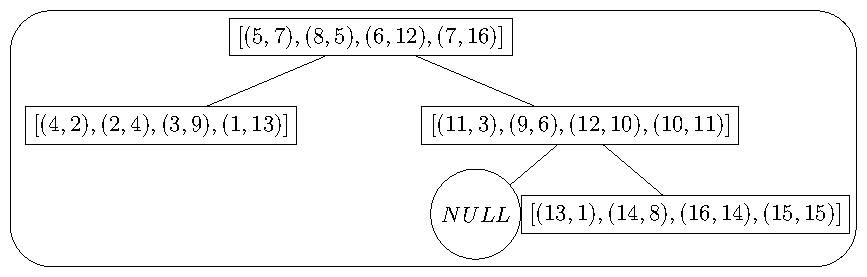
\includegraphics[scale=1]{bst.pdf}
\subsection{Algorithm : }
\begin{itemize}
\item[\bf STEP 1 : ]
Start
\item[\bf STEP 2 : ]
If($x_2 - x_1 < 2*(Log[n]) $, traverse elements in this range of x and return the points satisfying $y > y_{bottom}$. \\*
else Initialise variables node\_i to the x value of nearest node ahead of $x_1$ and node\_j to the x value of nearest node behind $x_2$.
\item[\bf STEP 3 : ]
Find the elements satisfying $y > y_{bottom}$ in the x range $x_1$ to node\_i and in x range node\_j to $x_2$, and report them.
\item[\bf STEP 4 : ]
Find the elements satisfying $y > y_{bottom}$ in the x range node\_i to node\_j and report them.
\item[\bf STEP 5 : ]
Stop.
\end{itemize}
\subsection{Pseudo Code : }
Report\_points($x_1,x_2,y_bottom$)	\\*
\{			\\*
	\hspace*{1cm}if($ x_2-x_1 <2*(Log[n])$) \\*
	\hspace*{2cm} Locate the required x range in the BST. \\*
	\hspace*{2cm}Report elements between that x range satisfying $y > y_{bottom}$ using binary search \\*
	\\*
	\hspace*{1cm}else if($x_1$ and $x_2$ exists in data points)\\*
	\hspace*{2cm} Locate the required x range in the BST. \\*
	\hspace*{2cm}Report elements between that x range satisfying $y > y_{bottom}$ using binary search \\*
	\\*
	\hspace*{1cm}else \\*
	\hspace*{1cm}node\_i $ \longrightarrow $ x value of the nearest node ahead of $x_1$ \\*
	\hspace*{1cm}node\_j $ \longrightarrow $  x value of the nearest node before $x_2$ \\*
	\hspace*{1cm}report\_i $ = $ Report\_points($x_1$, node\_i, $y_{bottom}$)		\\*
	\hspace*{1cm}report\_j $ = $ Report\_points(node\_j, $x_2$, $y_{bottom}$)		\\*
	\hspace*{1cm}report\_rest $ = $ Report\_points(node\i, node\j, $y_{bottom}$)		\\*
\}	 
\subsection{Space Complexity : }
	The data structure we invented, is a BST of size N*(augmentation size).\\*
Therefore, space used is $N * Log[n]$= n. (Refer Sub section Data Structure Design).
Implying space complexity is O(n).
\subsection{Time Complexity : }
\subsubsection{Query Time : }

\subsubsection{Pre-processing Time : }
\begin{itemize}
\item The first sort based on x coordinates requires O(n*Log[n]).
\item 
\item
\item

\end{itemize}
\end{document}
